\chapter{Evolutionary Algorithms} % top level followed by section, subsection

%: ----------------------- paths to graphics ------------------------

% change according to folder and file names
\ifpdf
    \graphicspath{{2/figures/PNG/}{2/figures/PDF/}{2/figures/}}
\else
    \graphicspath{{2/figures/EPS/}{2/figures/}}
\fi

%: ----------------------- contents from here ------------------------

%\begin{flushright}
%Life results from the non-random survival 
%\linebreak
%of randomly varying replicators.
%\linebreak
%Richard Dawkins 
%\end{flushright}
\section{Introduction - Overview of Evolutionary Algorithms}
Variations of stochastic optimization methods inspired and/or based on Darwin's theory of evolution on the origin of species \cite{Darwin} have been proposed. Hereafter, all these methods along with their variants will be referred to as Evolutionary Algorithms (EAs). The increasing power of modern computational platforms and its availability with relatively low cost, combined with algorithms capable to exploit their capabilities,  allowed EAs, combined with existing analysis tools, to be routinely used as industrial design tools.     

Generally, an EA is a stochastic optimization method that maintains a population of individuals $P^g=(\vec{x}_1,...,\vec{x}_{\lambda}),~\lambda \ge 1$ for each generation $g$. Each individual $\vec{x}$ represents a potential solution to the optimization problem in hand and must be evaluated to obtain a measure of its "fitness" or "cost", according to user-defined objective functions. Then, the population of the next ($g+1$) generation is formed by selecting the more fit individuals (to be referred to as parents) and evolve them by applying the so-called evolution operators (recombination, mutation, etc.) that mimic the evolution of species. The new population (to be referred to as offspring) is expected to better fit to the environment, determined by the selected objective function(s).     

The first attempts to use EAs as problem solving techniques is dated back to mid-50s and can be found is separate works presented by Friedberg, Brernermann and Box. Friedberg cite(1958 and 1959) presented an EA aiming at creating a program to perform a given task; though quite premature, this was in fact an ancestor of evolutionary programming (see below). During the same period of time, Bremermann (cite Bremermann 1962) was among the first to apply EAs in numerical optimization problems, for linear and convex problems as well as the solution of nonlinear systems of equations. Box proposed the use of EAs as a method for improving industrial processes and increasing industrial productivity (cite Box 1957, Box and Draper 1969). By that time, these first attempts were treated with considerable skepticism. However, during the next decade, methods which initiated the three key-classes of EAs, namely evolutionary programming (EP), evolutionary strategies (ES) and genetic algorithms (GA), have been proposed.

EP was proposed by L. J. Fogel by mid-60s  (cite fogel 64,66,68). EP was developed by considering machine learning tasks by means of finite state machines (FSM\footnote{A finite-state machine (FSM) is a mathematical model used to design computer programs and digital logic circuits. FSM is an abstract machine that can be in one of a finite number of states.}). The optimization problem was  initially defined as evolving an algorithm (program) for predicting arbitrary time series.  In EP  \cite{Fogel}, offspring are created by randomly mutating each parent, for producing one offspring. The offspring with the greatest payoff is, then, retained to become a parent in the next generation. EP was successfully applied to problems in prediction identification, automatic control and pattern recognition. Until mid-80s, EP was confined to the FSM representation. In 1986, though, EP was extended (Fogel and Fogel 1986) to alternative representations including ordered lists for the travelling salesman problem and real-valued vectors for continuous function optimization. Later, a self-adaptative EP (Fogel and Fogel 91,92) was proposed by including mutation variance in the evolution procedure.

The first ES was proposed in 1965 by Rechenberg using discrete, binomially distributed mutations (centered at the parent's position) and just a single parent and single offspring per generation. Later, ES was furthered developed both by Rechenberg (phd thesis 1971) and Schwefel (phd thesis 1975), via introducing recombination and adaptive mutation \cite{Rechenberg}. Using real-valued representation of the optimization variables, mutation is performed by adding a normally distributed random value to them. The introduction of recombination as an additional evolution operator for creating offspring, which was impossible with just a single parent, led to the so-called multi-membered ES. This led to the $(\mu, \lambda)ES$ i.e. an ES with $\mu$ parents and $\lambda$ offspring. One of the most successful variance of ES is the covariance matrix adaptation ES (CMA-ES) (cite Hansen N, Müller SD, Koumoutsakos P (2003)). CMA is used to update the covariance matrix of the multivariate normal distribution, which the candidate solutions are sampled from. CMA-ES was found to be particularly useful in cases where the objective function was ill-conditioned and the optimization variables non-separable (N. Hansen and A. Ostermeier. Completely derandomized self-adaptation in evolution strategies 2001 , N. Hansen and A. Ostermeier. Convergence properties of evolution strategies with the derandomized covariance matrix adaptation: The (μ/μI , λ)-CMA-ES. In Proceedings of the 5th European Congresson Intelligent Techniques and Soft Computing 1997).  

GA was initially proposed from Holland in 1962 (cite holland 1962 \cite{holland_1975}) as an evolution emulating tool for the understating of the underlying principles
of adaptive systems \footnote{Systems that are capable to undergo self-modification in response to their interactions with the environment which they must function in.}. This gave Holland a different focus compared to other contemporary researchers in the field of EAs and reflected upon the algorithmic nature of GA in the sense that the mechanisms of reproduction and inheritance were based on operators well known from genetics \footnote{Genetics is a branch of biology, the science of genes, heredity, and of the variation in living organisms} such as mutation, crossover and inversion. In addition, the representation of the objects to be evolved as binary strings in direct analogy to the genetics genome. The binary string representation is one of the distinctions between ES and GA, considered as important at least in the early stages of their lives.  
 
Genetic programming (GP) was proposed, later, by Crammer in mid-80s \cite{cramer85} and, then, improved by Koza \cite{Koz94} aiming at the automated design of computer programs with the ability to perform a given computational task. In GP, individuals (computer programs) are represented as tree structures \footnote{A tree structure can represent graphically the hierarchical nature of an object. Tree structures start from the so called "root" node, which is the highest in hierarchy. Lines connecting elements are called "branches" and the elements themselves "nodes". The lowest in hierarchy nodes  "end-nodes" or "leaves". } where each node is given an operator function and each terminal node an operand. Representing programs in this way offers easy evaluation and makes the application of evolution operators possible, in the sense that recombination can take place by exchanging nodes between the parents and mutation by randomly replacing a node. 

In the Parallel CFD \& Optimization Unit of NTUA (PCOpt/NTUA), GA and ES are both represented in a generalised $(\mu,\lambda)EA$ scheme (cite Giotis Kampolis Karakasis).  The $(\mu,\lambda)EA$ main characteristics are the population-based evolution and the fact that the inheritance of candidate solution features is based on probabilistic criteria and decisions made upon a fitness or cost function quantifying the ability of each individual to survive in the environment. Evolution, from each generation to the next, fig~\ref{EA}, is achieved through the so-called evolution operators (recombination, elitism, mutation and parent selection). The generalised $(\mu,\lambda)EA$ scheme, which is used and enhanced in this PhD thesis, can be transformed to either a conventional ES or conventional GA by adjusting the algorithmic settings and the optimization variable representation (binary or real), accordingly.  

The two main advantages of EAs are: a) their ability to avoid local optima and locate the desirable global optimum and b) that they may accommodate any ready-to-use analysis software without having access to its source code. The only prerequisite for carrying out an EA-based optimization is the availability of a evaluation software (even commercial, i.e. considered as a black–box tool within the optimization loop) for the specific optimization  and well defined design variables and objective functions. However, the need to evaluate all individuals in the population for assigning fitness or cost values to them is the weak point of all EAs used in problems which the evaluation of each candidate solution is computationally demanding. Optimization in aerodynamics or hydrodynamics which is based on expensive Computational Fluid Dynamics (CFD) software is a typical example.  This increases noticeably the optimization turn-around time and, often, makes the whole process non-affordable for industrial use. To overcome this weakness, several techniques have been proposed in the literature. These  are classified in those aiming at reducing the optimization turn-around time by performing concurrent evaluations of the population members on a multi-processor platform and those reducing the number of evaluations needed to reach the optimal solution(s). Both techniques can certainly be used in combination.   

A Parallel Evolutionary Algorithm (PEA) (cite pfd kampolis Vera giotis karakasis + 3ed party) is an EA adapted to take advantage of the availability of a multi-processor platform, in order to reduce the optimization turn-around time. PEAs can be classified into single- and multi-population EAs. In a single-population or panmictic EA, each population member can, potentially, mate (recombination) with any other; standard way of parallelization is the concurrent evaluation scheme, with centralized selection and evolution (the so called master-slave model). A multi-population EA handles partitioned individual subsets, according to a topology which might directly map onto the parallel platform and employs decentralized evolution schemes; these can be further classified to distributed (cite giotis, marios, kampolis + 3ed party) and cellular EAs, (cite Alba, Enrique, Dorronsoro, Bernabe 2008), depending on the subpopulations’ structure and granularity. 

All the aforementioned PEAs refer to synchronous EAs, in which the use of the multi-processor platform is restricted to the concurrent evaluation of candidate solutions, without altering the sequential nature of evolution in an EA. This creates a synchronization barrier at the end of each generation where a number of processors may remain idle while waiting for the remaining candidate solutions of the generation to be evaluated.  In order to minimize (practically eliminate) the idle time of processors, asynchronous EA (AEA) (from others+\cite{LTT_2_040}) have been developed. An AEA overcomes the sequential nature of evolution by applying the evolution operators to a number of strongly interacting (overlapping) demes, which may optimally use all the available processors.     

A metamodel-assisted EA (MAEA) is the EA that employs low-cost surrogate evaluation models, i.e. the so called "metamodels", as often as possible, during the optimization. This decreases substantially the number of calls to the computationally expensive, problem-specific evaluation code (CFD). Polynomial regression, artificial neural networks, Gaussian processes etc. have all been used as metamodels. Schemes based on different interactions between the metamodel and the problem-specific evaluation tool have been proposed in the literature \cite{KEANEbook,LTT_2_020,Jin2002,LTT_2_027}. MAEA implementation can be classified in two basic categories, depending on whether the metamodel(s) is/are trained before (off–line) or during (on–line) the evolution. Additionally global (i.e. a single metamodel for the entire search space) and local (i.e. a number of metamodels valid over different parts of the search space) metamodels can be used.

On the other hand, hierarchical EAs (HEAs) or MAEAs (HMAEA)(phd mariou + kamp +3ed party) are build based on a small number of interconnected levels. On each level, different search methods, different evaluation software and/or different sets of design variables can be employed. One- or two-way inter-level communication schemes can be used. On levels employing an EA-based search, a PEA or MAEA or both can be employed. Multi-level optimization algorithms can, generally, be classified as follows (REF se PARCFD2007):

(a) \emph{Multi-level Evaluation,} where each level is associated with
a different evaluation software. The lower levels are responsible
for detecting promising solutions  on low CPU cost, through less
expensive problem--specific evaluation models, and
delivering them to the higher level(s). There, evaluation models of
higher fidelity and CPU cost are employed and the immigrated
solutions are further refined. The availability of low- and  high- fidelity problem-specific (CFD) tools can thus be exploited.

(b) \emph{Multi-level Search,} where each level is associated with a
different search technique. Stochastic methods, such as EAs, are
preferably used at the lower levels for the exploration of the
design space, leaving the refinement of promising solutions to
gradient-based methods on the higher level(s). Other
combinations of search tools are also possible. Memetic algorithms (ref dika mas + 3ena) is a class of multilevel search that combines global and local search methods, aiming at improving the quality of
promising solutions.


(c) \emph{Multi-level Parameterization,} where each level is
associated with a different set of design variables. On the lowest
level, a subproblem with just a few design variables is solved. On
the higher levels, the problem dimension increases. The most detailed parameterization is used on the highest level.


\figuremacroW{EA}{EA schematic representation }{Schematic representation of the EA. Each population is derived by the previous one via evolution operators, such as parent selection, crossover and mutation }{0.8}

\section{Optimization problems - Definitions}
Any optimization problem with $M$ objectives (cast in the vector form $\vec{F}$) and $K$ constraints (cast in the vector form $\vec{C}$) can be formulated as:
\begin{align} 
   &min ~ \vec{F}(\vec{x})=(f_1(\vec{x}),f_1(\vec{x}),...,f_M(\vec{x}))\in \Re^{M} \nonumber \\
   &\mbox{subject to} ~ c_k(\vec{x})\leq d_k, ~~~~~ k =1,K
\label{OptimIN}
\end{align}
where $\vec{x}\in X \!\leq\! \Re^{N}$ is the design vector and $X$ the design space. If equality constraints $ c^*(x)=d^* $ are to be imposed, these can be transformed into inequality constraints $ c(x)=\Vert c^*(x)-d^*\Vert \leq d $ where $ d \in \Re $ is an infinitessimally small number. If $M \!> \!1$ problem \ref{OptimIN} represents a multi-objective optimization (MOO) problem ; in such a case, the notion of Pareto dominance \cite{Zitzler2000} is used to associate a scalar cost value to each individual, based on which an algorithm solving single-objective optimization (SOO) problems can be employed. In MOO problems, a single run of an EA is capable of delivering a Pareto front of non-dominated individuals, rather that a single "optimal" solution, standing for a compromise among the various objective functions. 

\subsection{Multi-Objective Optimization and EAs}
\label{MOOini}
In contrast to SOO, where the scalar cost function, which defines the survival of candidate solutions from generation to generation, is derived directly from the objective function (depending on whether minimization or maximization problems are to be solved) a MOO problem solver handles a vector of objectives. Therefore, a technique to transform this vector to a scalar cost value is needed, in order to rely on the same SOO problem solving EA. Several techniques for handling this problem exist in the literature \cite{CoCo99,coe02,Miett99}. The most commonly used among them concentrate the objective functions into a scalar cost function either by associating weights to each one of them or by accounting for the distance between the candidate solution and a user-defined ideal design or, even, using ranking techniques based on the notion of Pareto dominance (see below). In this PhD, all MOO problems are handled using techniques relying on Pareto dominance criteria. Different implementations of Pareto dominance based techniques exist in the literature among which let us mention MOGA \footnote{Multi-objective Genetic Algorithm.} \cite{Fon93}, NPGA \footnote{Niched Pareto Genetic Algorithm.} \cite{horn94}, NSGA \footnote{Non-Dominated Sorting Genetic Algorithm.} \cite{Sri1995}, NSGAII \cite{Deb00a}, SPEA \footnote{Strength Pareto Evolutionary Algorithm.}\cite{ZiTh98}, SPEAII \cite{Zitz02,Zitz01}, PAES \footnote{Pareto Archived Evolution Strategy.} \cite{knowles99} and PESA \footnote{Pareto Envelope-based Selection Algorithm.} \cite{corne00}. The definitions of Pareto dominance and Pareto optimality, on which the aforementioned techniques rely on, follow:

\paragraph{Pareto Dominance:} Solution $\vec{x}_1$ dominates solution $\vec{x}_2$ ($\vec{x}_1\prec\vec{x}_2$) if and only if $\vec{F}(\vec{x}_1)$ is partially less than $\vec{F}(\vec{x}_2)$, i.e.
\begin{eqnarray}
    \vec{x}_1\prec\vec{x}_2 \Leftrightarrow (\forall i :  f_i(x_1) \leq f_i(x_2))\wedge (\exists _i : f_i(x_1) < f_i(x_2)),~~~~i=1,M
   \label{pareto_eq} 
\end{eqnarray}

\paragraph{Pareto Optimality:} Solution  $\vec{x}_1 \in X$ is a Pareto optimal solution with respect to $X$ if and only if there is no $\vec{x} \in X$ that dominates $\vec{x}_1$, or 


\begin{eqnarray}
    \nexists\vec{x}:\vec{x}\prec\vec{x}_1, ~~~~ \vec{x},\vec{x}_1\in X \!\leq\! \Re^{N}
\end{eqnarray}
 
\figuremacroW{Pareto2}{Pareto dominance}{Schematic representation of Pareto dominality. $\vec{x}_1$ is a Pareto optimal solution since it is not dominated by any other solution. Furthermore $\vec{x}_1$ itself dominates all individuals located in the grey box.}{0.5}

In fig. \ref{Pareto2}, a schematic representation of the Pareto optimality in a group of individuals is presented. A minimization problem with two objective functions, $f_1$ and $f_2$, is considered. Black circles denote the front of non-dominated individuals whereas the empty circles denote dominated individuals. In the sake of clarity the part of the objective space which is dominated by $\vec{x}_1$ is highlighted in grey. Individuals located in the grey area are dominated, at least, by $\vec{x}_1$. 

A detailed presentation of three techniques (SPEA,SPEAII and NSGAII) used in this thesis follow in section \ref{MOO}.

\subsection{Constrained optimization and EAs}
\label{COPini}
In engineering, almost all optimization problems are subject to constraints which split the design space in feasible and infeasible regions. EAs may handle constraints through a) the use of penalty functions \cite{Deb00,morales98} assigning greater chances to survive to individuals satisfying the constraints \cite{powell93}, b) the conversion of constraints into objectives \cite{surry95,surry97} and/or c) the use of correction operators \cite{mich94}. Detailed survey on this subject can be found in \cite{mich96,coello02}. In the present thesis, penalty functions are used as presented in section \ref{COP}. 

\section{The Evolutionary Algorithm SYstem (EASY)}
EASY is a generic optimization platform which implements the $(\mu,\lambda)EA$. EASY has been developed by PCOpt/NTUA (cite phd kampolis, giotis, karakasis) and the techniques proposed in this thesis have all been built on EASY. EASY supports multilevel optimization in all its possible forms and is Grid/Cluster-computing enabled, based on the DRMAA library. A detailed analysis of the implemented $(\mu,\lambda)EA$, considered as the background optimization method in this thesis, follows.  


\subsection{The $(\mu,\lambda)$EA}
\label{MLEA}
Each generation, denoted by the superscript $g$, of the $(\mu,\lambda)$EA is associated with three dynamically updated populations: the offspring $P_{\lambda}^g$ population with $\lambda$ offsprings, the parent $P_{\mu}^g$ population comprising $\mu$ parents and the elite $P_{e}^g$ population with $e$ elites. $P_{e}^g$ contains all or some of the currently best individuals. Depending on the design variables coding (binary, binary Gray or real), appropriate evolution operators must be applied. 

The background $(\mu,\lambda)$ EA in use (cite Giotis 2003):
\begin{itemize}
\item[]{\bf Step 1:}  (Initialization) $g=0$, $P_{e}^{g-1}=0$ and $P_{\mu}^g=0$. All $P_{\lambda}^g$  members are initialized using a pseudo-random number generator, in accordance to the user-defined lower and upper bounds. Optional injection of user defined individuals, such as existing designs from the same or a similar problem, in the initial population is possible. 
\item[]{\bf Step 2:}  (Evaluation) All individuals in $P_{\lambda}^g$ must be evaluated using the problem-specific evaluation tool. Below, this will also be referred to as exact evaluation tool to make the distinction as to whether this or a cheaper surrogate model of it is to be used. The evaluation step, generally, is time-consuming and yields the vectors $\vec{F}(\vec{x}) \in \Re^{M} $ for each $\vec{x} \in P_{\lambda}^g$.
\item[]{\bf Step 3:}  (Cost assignment) For each $\vec{x} \in P_{\lambda}^g \cup P_{\mu}^g \cup P_{e}^g$, a scalar cost $\Phi(\vec{x})$ value is assigned as a function of $\vec{F}(\vec{x})$. In SOO $\Phi(\vec{x})=F(\vec{x})$.
\item[]{\bf Step 4:}  (Elite selection) The $e^*$ non-dominated (for MOO) or best for (SOO) individuals in $P_{\lambda}^g \cup P_{e}^{g-1}$ are selected to enter $P_e^g$. If $e^* > e$, a thinning operator must be applied to remove $e^* - e$ individuals.     
\item[]{\bf Step 5:}  (Elitism) A small number of elite individuals (selected, at random form $P_e^g$) replace the worst members of $P_{\lambda}^g$.  
\item[]{\bf Step 6:}  (Parent selection) The new parent population $P_{\mu}^{g}$ is selected from $P_{\mu}^{g-1}$ and $P_{\lambda}^g$ by taking into account the allowed maximum age  $k$ of individual, measured in generations, for each parent. Symbolically, $P_{\mu}^{g}=S(P_{\mu}^{g-1},P_{\lambda}^g,k)$ 
\item[]{\bf Step 7:}  (Recombination and mutation) The next generation of the offspring population $P_{\lambda}^{g+1}$ is derived from 
$P_{\mu}^{g}$  by applying the recombination and mutation operators. Recombination $\mathcal{R}(P_{\mu}^{g})$ is the process of combining the genotype of a number ($n$) of parents to create an offspring (see \ref{evOps}). The recombination operator is used $\lambda$ times, using differed sets of $n$ parents randomly selected from $P_{\mu}^{g}$,  to create the $\lambda$ new offspring. Next step for the formation of $P_{\lambda}^{g+1}$ is the application of the mutation operator. Mutation is a process that, with a small probability, randomly alters parts of the individual genotype. Symbolically, $P_{\lambda}^{g+1} = \mathcal{M}(\mathcal{R}(P_{\mu}^{g}))$ (see \ref{evOps}).
\item[]{\bf Step 8:}  (Stopping check) Unless any of the stopping criteria is met, return to $step 2$.
\end{itemize}

\begin{table}[htdp]
\centering
\begin{tabular}{lr} 
\hline
\hline
Number of objectives & M\\
Number of design variables & N\\
Number of constraints   & K\\
\hline
Candidate solution   & $\vec{x}$\\
Objectives vector  & $\vec{F}$\\
Constraints vector  & $\vec{C}$\\
Cost value & $\Phi$ \\
\hline
\hline
\end{tabular}
\caption[GEA nomenclature]{The nomenclature of the ($\mu,\lambda$)EA.}
\label{GEA nomenclature} 
\end{table}


\subsubsection{Evolution operators}
\label{evOps}
The evolution operators employed in EASY are the parent selection, the recombination, the mutation and the elitism operator. These are further discussed below. 
   
\paragraph{Parent selection:}
The parent selection operator selects the members of $P_{\mu}^{g}$ from a set of individuals; in EASY, based on the previous algorithm (Step 6) this is the union of $P_{\mu}^{g-1}$ and $P_{\lambda}^g$. The most common parent selection techniques are presented: 
\begin{itemize}
\item[]{\bf a) Proportional selection.} Each member of the aforementioned set is given a probability to become a parent, which is inversely proportional to its cost value $\Phi$. Recall that a minimization problem is to be solved. This scheme is, practically, implemented via a roulette wheel algorithm. Each and every set member is associated with a slot on the roulette wheel, where the size of the slot respects its probability to become a parent. The roulette will is used $\mu$ times so as to create the $\mu$ parents.  
\item[]{\bf b) Linear ranking.} In linear ranking, the set members are sorted according to their $\Phi$ values and placed in a sorted list. The probability of each one of them to become a parent depends linearly only on its position in the aforementioned list and not on the $\Phi$ values themselves.
\item[]{\bf c) Probabilistic tournament selection.}
In probabilistic tournament selection \cite{goldberg1991}, a number of randomly chosen individuals are selected from the aforementioned set and with a user defined, typically high, probability the best individual from this group is selected as parent. This process is repeated $\mu$ times so as to select the required $\mu$ parents without replacement. Common parameters for tournament selection is the tournament size i.e. how many individuals participate in each tournament and the probability to select the best of them. Typical values are $2$ or $3$ individuals per tournament and $80\%$-$95\%$ probability to select their best.
\end{itemize}

\paragraph{Recombination:}
Since the first appearance of EAs, there has been numerous discussions about the merits of recombination as an evolution operator in EAs. In general, the purpose of recombination is to increase the probability of offspring to be fitter than its parent(s). Recombination algorithms can be classified depending on design variables coding, as follow: 

In EAs based on {\bf binary coding}, the {\bf recombination} operator undertakes the exchange of pieces of the binary string that describes the design vector between the parents in order to create an offspring. In EASY, the following types of binary coding recombination exist:
\begin{itemize}
\item[]{\bf a) One-point recombination.} 
In the one-point binary recombination, with $\rho$ parents per offspring, the binary string is divided into $\rho-1$ parts of equal length in binary digits. Then $\rho$ parents are selected at random from the $P_{\mu}^{g}$ set and $(\rho-1)$ pairs of parents are formed, in all of which the first parent should participate. If the first parent is denoted by 1, the $(\rho-1)$ pairs are: $(1,2),(1,3),...,(1,\rho)$. 
%The pairings take place serially between the lead parent (parent with higher $\Phi$) and the $i^{th} \in [1,\rho-1] $ one. 
For each one of the $(\rho-1)$ pairs of the chromosome, a random integer $\mathcal{X}$ determines the corresponding crossover point. The offspring is formed by combining the left part of the string part taken from the first parent and the right one from the other parent, based on the aforementioned pairings. A three-parent example ($\rho=3$) is presented in fig \ref{1px}.
\begin{figure}[h!]
\begin{minipage}[b]{1.0\linewidth}
 \centering
 \resizebox*{11cm}{!}{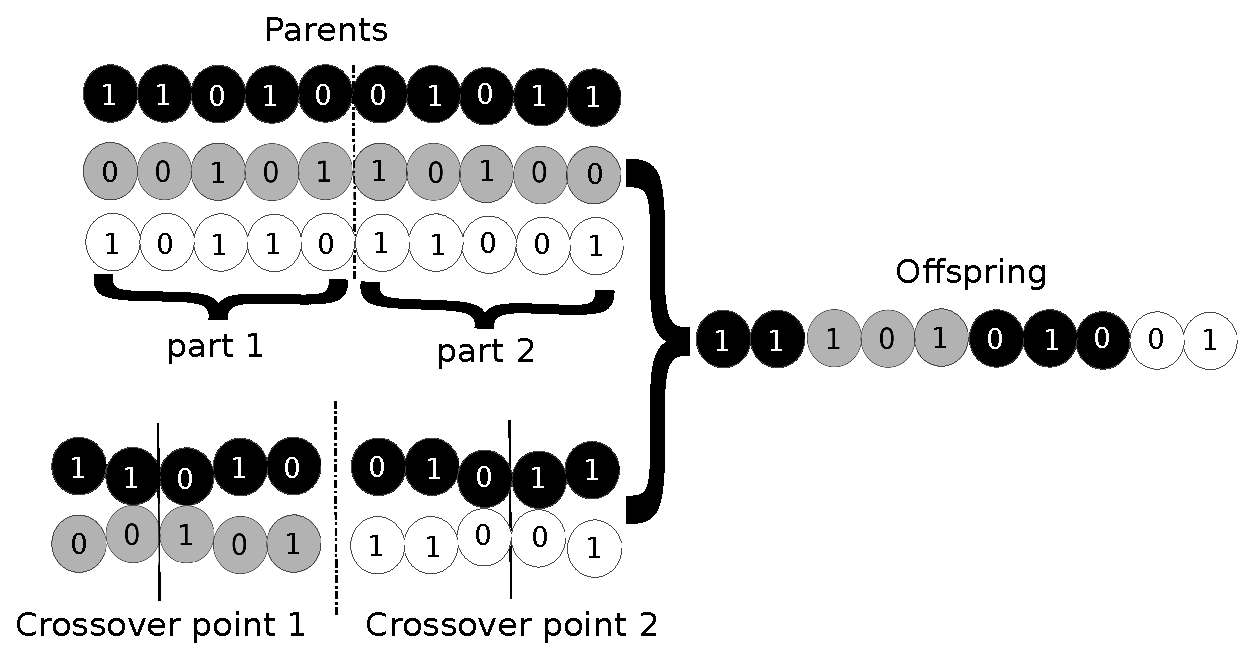
\includegraphics{onepointbinary.eps}}
\end{minipage}
\caption{One-point binary coding recombination with $\rho=3$. In this case, the chromosome is divided in two parts ($\rho-1 = 2$) and two vertical cuts are created by the random number generator.} 
\label{1px}
\end{figure}

\item[]{\bf b) Two-point recombination}. This scheme is similar to its one-point counterpart, the only difference being that two crossover points are used ($\mathcal{X}_1~\&~\mathcal{X}_2$). A two-parent example is illustrated in fig \ref{2px}.

\begin{figure}[h!]
\begin{minipage}[b]{1.0\linewidth}
 \centering
 \resizebox*{11cm}{!}{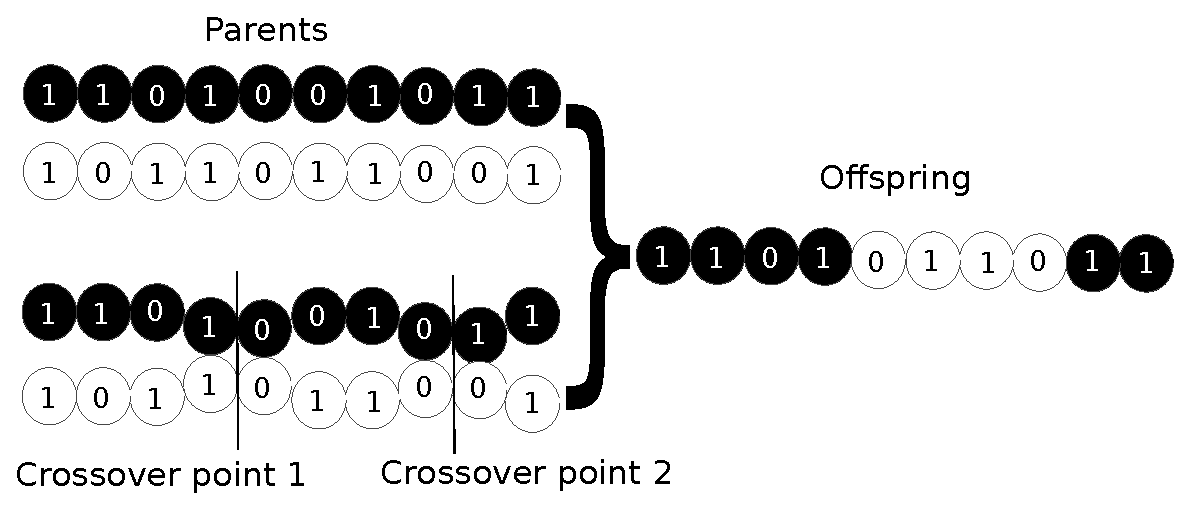
\includegraphics{twopointbinary.eps}}
\end{minipage}
\caption{Two-point binary coding recombination with $\rho=2$. In this simple case, the chromosome is handled as a whole ($\rho-1 = 1$) and two vertical cuts are created by the random number generator.} 
\label{2px}
\end{figure}

\item[]{\bf c) One- or two-point recombination per design variable}. Here, the aforementioned one- and two-point recombination schemes are separately applied to the parts  of the binary string that correspond to each design variable.  
\end{itemize}
  
Using the {\bf real coding} of the design variables $\vec{x}$ the {\bf recombination} operator must be applied directly on to the real-valued design variables. In EASY, this is carried out as follows:  

\begin{itemize}
\item[]{\bf a) One- or two-point recombination.} The one- and two-point recombination schemes as proposed with binary coding, can also be adapted to real coding by exchanging  pieces of the design vector $\vec{x}$ instead of pieces of binary strings. The randomy selected crossover variable is the only one to be affected by both parents according to a randomly generated weight $r$. A one-point, two parents example is presented in fig \ref{1pxreal}.

\begin{figure}[h!]
\begin{minipage}[b]{1.0\linewidth}
 \centering
 \resizebox*{11cm}{!}{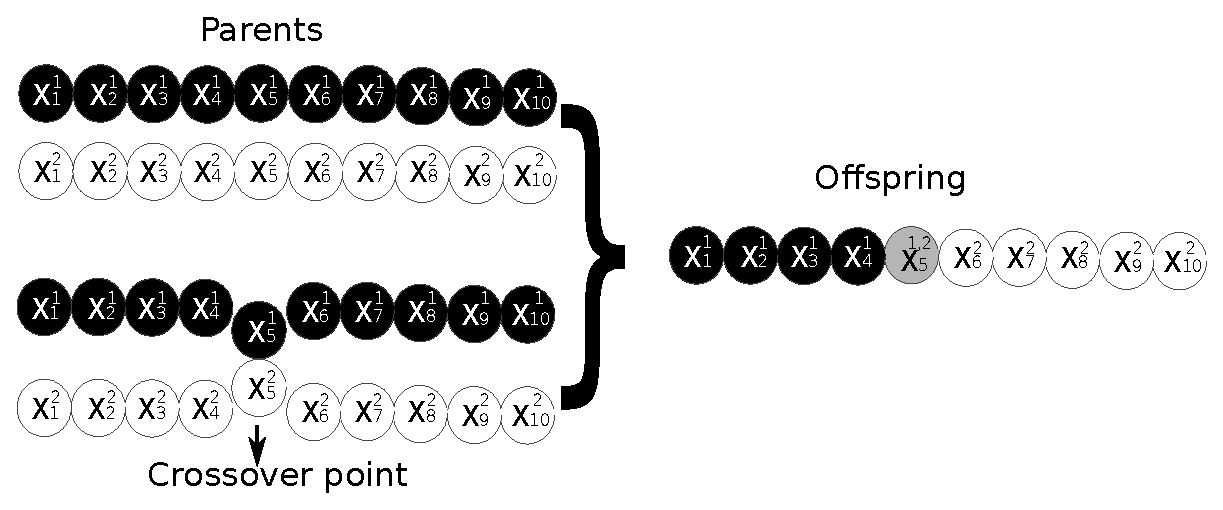
\includegraphics{pointreal.eps}}
\end{minipage}
\caption{One-point real coding recombination with $\rho=2$. Superscript denote the parent and subscript the design variables. The crossover variable (e.g. $5$) is selected at random. In the offspring this variable will be given by  $x_5^{1,2}=x_5^{1}+r(x_5^{2}-x_5^{1})$, where $r$ is a random number, uniformly distributed in $[0,1]$ ($r \in U(0,1)$).    
} 
\label{1pxreal}
\end{figure}
 
\pagebreak    
\item[]{\bf b) Discrete recombination.} In discrete recombination with $\rho$ parents each real-valued design variable in the offspring has $50\%$ probability to be copied either from the first parent $\vec{x}^1$ or a randomly chosen among the $\rho-1$ remaining ones $\vec{x}^{random}$. A three-parents example is presented in fig \ref{disc}.

\begin{figure}[h!]
\begin{minipage}[b]{1.0\linewidth}
 \centering
 \resizebox*{11cm}{!}{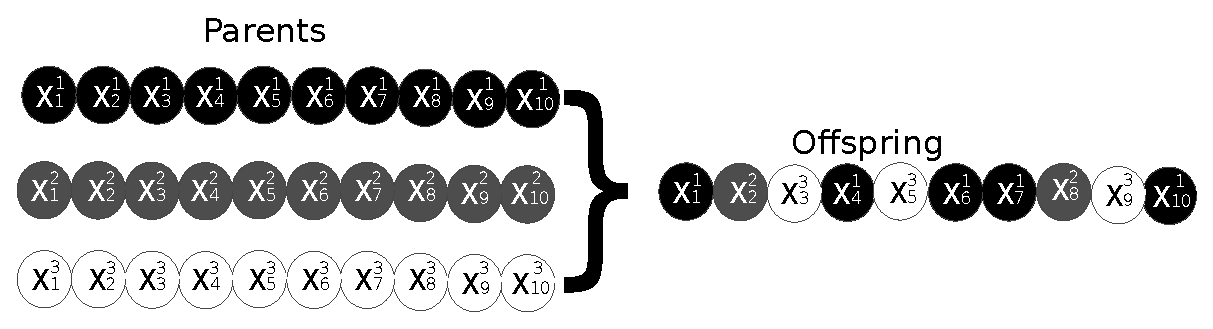
\includegraphics{discrete.eps}}
\end{minipage}
\caption{Discrete real coding recombination with $\rho=3$. $\vec{x^1}$ is the first parent.    
} 
\label{disc}
\end{figure}
    
    
\item[]{\bf c) Intermediate recombination}.  In intermediate recombination, each component of the offspring $\vec{x}$ is a linear combination of the first parent $\vec{x}^1$ and a randomly chosen among the $\rho-1$ remaining ones $\vec{x}^{random}$, namely
\begin{eqnarray}
\nonumber
\vec{x}=\vec{x}^1+r(\vec{x}^{random}-\vec{x}^1),~ r\in U[0,1]
\end{eqnarray}  
where a different random number is generated for each design variable.
 
\item[]{\bf d) Simulated binary crossover}. The so called simulated binary crossover (SBX) \cite{SBX1} was designed aiming at recreating the one-point binary recombination properties of a) average property \footnote{The average of the decoded variable values is the same
before and after the crossover operation.} and b) spread factor property\footnote{Spread factor ($\beta$) is defined as the ratio of the spread of offspring to that of parents. Contracting, expanding or stationary recombination correspond to $\beta <1$, $\beta >1$ or $\beta =1$ respectively. The spread factor property states that probability of occurrence of spread factor $\beta \approx 1$ is more likely than any other $\beta$ value. }\cite{SBX1}. The offspring $\vec{x}$ is generated as follows;
\begin{eqnarray}
	\vec{x}={\left\{ 
	\begin{array}{ll}
    \vec{\overline{x}} - \frac{\beta}{2} (\vec{x}^{random}-\vec{x}^1)~~,\mbox{if $r < 0.5$}\\
	\vec{\overline{x}} + \frac{\beta}{2} (\vec{x}^{random}-\vec{x}^1)~~,\mbox{if $r \geq 0.5$}
    \end{array} \right. }
    \label{sbxx}
\end{eqnarray}  
where $r\in U[0,1]$,$\vec{x}^1$ the first parent, $\vec{x}^{random}$ is a randomly selected among the $\rho-1$ remaining parents, $\vec{\overline{x}}$ is the middle point between $\vec{x}^{1}$ and $\vec{x}^{random}$ and 
\begin{eqnarray}
	\beta={\left\{ 
	\begin{array}{ll}
    (2r)^{n}~~~~~~,\mbox{if $(r \leq 0.5)$}\\
	\left(\frac{1}{2r}\right)^{n+2}~~,\mbox{if $(r > 0.5)$}
    \end{array} \right. },~~~~ \mbox{fig.\ref{sbx}}.
    \label{betasbx}
\end{eqnarray}

Because $r\in U[0,1]$, the probability distribution of $\beta$ can be plotted for various $n$ based on eq.\ref{betasbx} (fig.\ref{sbx}-left). Based on the $\beta$ probability distribution and eq.\ref{sbxx}, the probability distribution of offspring appearance on the design space as a function of $n$ and the parents can be plotted (fig.\ref{sbx}-right for a 1d problem and fig.\ref{sbx2} for a 2d problem). In general higher $n$ values increase the probability of $\beta \approx 1$, which inturn increases the probability of creating near-parent offspring (spread factor property). Together with the symmetrical offspring probability distribution with respect to $\vec{\overline{x}}$ (average property) "SBX" can simulate the one point binary crossover ergo.    

\begin{figure}[h!]
\begin{minipage}[b]{0.5\linewidth}
 \centering
 \resizebox*{7cm}{!}{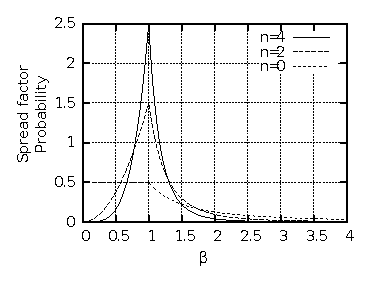
\includegraphics{SBX.eps}}
\end{minipage}
\begin{minipage}[b]{0.5\linewidth}
 \centering
 \resizebox*{7cm}{!}{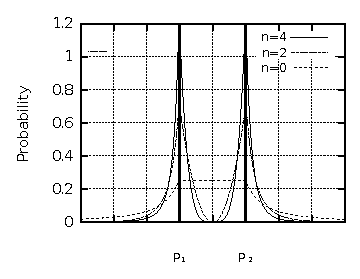
\includegraphics{SBXparents.eps}}
\end{minipage}
\caption{The offspring probability distribution of a 1D problem using SBX recombination with various $n$ is plotted as a function of the parents $P_1$ and $P_2$ (right). The corresponding probability distributions of $\beta$ are plotted left. Increasing $n$ leads to higher probability of $\beta \approx 1$.  }
\label{sbx}
\end{figure}

\begin{figure}[h!]
\begin{minipage}[b]{0.5\linewidth}
 \centering
 \resizebox*{7cm}{!}{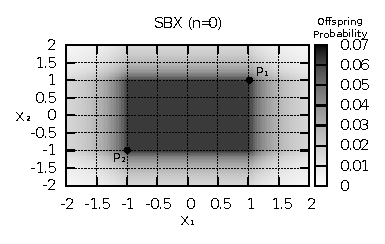
\includegraphics{SBX3dparents0.eps}}
\end{minipage}
\begin{minipage}[b]{0.5\linewidth}
 \centering
 \resizebox*{7cm}{!}{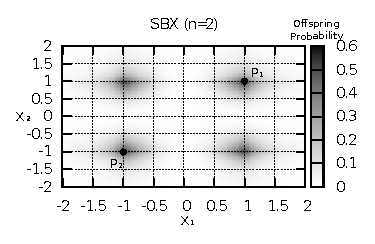
\includegraphics{SBX3dparents2.eps}}
\end{minipage}
\caption{The offspring probability distribution in a 2D optimization problem using SBX recombination for $n=0$ (left) and $n=2$ (right) is presented. The recombination uses two parents $P_1(1,1)$ and $P_2(-1,-1)$.}
\label{sbx2}
\end{figure}
\end{itemize}
  
\paragraph{Mutation,}
In an EA scheme the purpose of mutation is to introduce and preserve diversity in the population. Thus, mutation prevents the population from becoming homogenised prior to reaching the optimal solution, which would lead to slow or stagnated evolution. Mutation is applied to each offspring resulted from the recombination, subject to a small mutation probability $P_m$. Mutation, as recombination, depends also on whether binary or real coding is used.

In EAs based on {\bf Binary coding}, the {\bf mutation} is applied on each and every bit of the binary string. Each bit ca be flipped \footnote{Bit flipping is a state switch, from 0 to 1, or vice versa.}, with a probability $P_m$.      

\begin{figure}[h!]
\begin{minipage}[b]{1\linewidth}
 \centering
 \resizebox*{10cm}{!}{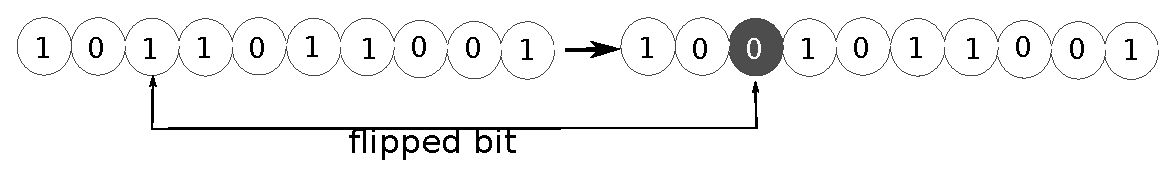
\includegraphics{mut.eps}}
\end{minipage}
\label{binarymut}
\end{figure}

\pagebreak
In {\bf Real coding mutation}, {\bf coding mutation} is applied on each real-valued component of $\vec{x}$. 

\begin{eqnarray}
	\vec{x}_m={\left\{ 
	\begin{array}{ll}
    \vec{x}~~~~~~~~~~,\mbox{if $(P_m > \vec{r})$}\\
	M(\vec{x},D)~,\mbox{if $(P_m \leq \vec{r})$}
    \end{array} \right. }
    \label{}
\end{eqnarray}
where $r\in U[0,1]$ and

\begin{eqnarray}
	M(\vec{x},D)={\left\{ 
	\begin{array}{ll}
    \vec{x}+D(g,\vec{U}-\vec{x})~,\mbox{if $(r_1 > 0.5)$}\\
	\vec{x}-D(g,\vec{x}-\vec{L})~,\mbox{if $(r_1 \leq r)$}
    \end{array} \right. }
    \label{}
\end{eqnarray}
where, $r_1\in U[0,1]$, $\vec{U}$ and $\vec{L}$ the vectors of upper and lower bounds of $\vec{x}$, accordingly, and  

\begin{eqnarray}
   D(g,y) = y r_2 (1-g/g_{max})^{0.2}
\end{eqnarray}
where $g_{max}$ the number of maximum generations and $r_2\in U[0,1]$. If the maximum number of evaluations is determined by the termination criterion, then $g/g_{max}$ should be replaced with $Ev/Ev_{max}$ where $Ev$ is the evaluation count and $Ev_{max}$ the maximum allowed number of evaluations.  

%\begin{eqnarray}
%	\vec{\sigma}=\frac{min(\mid \vec{x}-\vec{UB}\mid,\mid \vec{x}- \vec{LB}\mid)}{3} * (1-\frac{g}{g_{max}})^p
%	\label{sigmamut} 
%\end{eqnarray}
%where $\vec{UB}$ and $\vec{LB}$ the vectors of upper and lower bounds for the design variables respectively. $g$ the current generation and $g_{max}$ the maximum allowed generations.$p \simeq 0.2$.

%The first part of the eq.\ref{sigmamut} ensures that the mutated individual will respect the design variable bounds and the second part reduces exponentially eith $p$ the magnitude of $\vec{\sigma}$ as the generations advance.

%\begin{figure}[h!]
%\begin{minipage}[b]{0.5\linewidth}
% \centering
% \resizebox*{7cm}{!}{\includegraphics{Mut_1d.eps}}
%\end{minipage}
%\begin{minipage}[b]{0.5\linewidth}
% \centering
% \resizebox*{8cm}{!}{\includegraphics{Mut_2d.eps}}
%\end{minipage}
%\label{realmut}
%\caption{Examples of mutant probability distributions for one design variable left $x=0.4$ and two design variable right $\vec{x}=(0.4,0.9)$. For both cases $\vec{LB}=0$ and $\vec{UB}=1$.}
%\end{figure}

\paragraph{Elitism}
The purpose of elitism in EAs is to guarantee a monotonously improving course of evolution \cite{Back1996}. In EASY, the elitism operator is generalize with the use of a separate population $P_e^g$ updated each generation as described in ($\mu,\lambda$)EA (step 4) (see \ref{MLEA}). Furthermore, a number of user-specified elite individuals replace the worst members of the offspring population $P^g_{\lambda}$ before the parent selection operator takes place.
  
\subsection{MOO-EASY}
\label{MOO}
As mentioned in \ref{MOOini} a technique that transforms $\vec{F}$ into a scalar cost function $\Phi$ is required (eq. \ref{MOOeq}). The available in EASY techniques of SPEA, SPEAII and NSGAII are presented below.

\begin{eqnarray}
    \Phi(\vec{x})=\Phi(\vec{F}(\vec{x})) :\Re ^M \rightarrow \Re ^1 
	\label{MOOeq}
\end{eqnarray}

\paragraph{SPEA:}
SPEA was proposed in 1998 by Zitzler and Thiele \cite{ZiTh98} as a MOO cost assignment technique based on Pareto dominance. In SPEA eq.\ref{MOOeq} transformation takes place in two steps namely;
\begin{itemize}

\item[]{\bf Step 1:}  (Strength calculation) the strength of each member of the population $P$ is computed. Strength of the individual $i$ ($S_i$) is defined as the sum of the population members that are dominated or are equal to $i$ divided by the total number of the individuals in the population.  
 

\begin{eqnarray}
	S_i = \frac{\sum(j : j \in P \wedge i \prec j)} {\sum P}, ~~ \forall i \in P =P_{\lambda}^g \cup P_{\mu}^g \cup P_{e}^g  
\end{eqnarray}

\item[]{\bf Step 2:}  (cost calculation) the cost values for all population members are calculated as the sum of the strengths of the population members that dominate it.

\begin{eqnarray}
	\Phi_i = \sum _{j \in P \wedge i \prec j}(S_j)
\end{eqnarray}
\end{itemize}
  
 
\paragraph{SPEA II:}
SPEA II \cite{Zitz02,Zitz01} is an enhanced variant of SPEA, which incorporates density \footnote{A nearest neighbor density estimation technique is incorporated which allows a more precise guidance of the search process.} information. Thus improving the distribution of the individuals on the resulting Pareto front, traditional SPEA had a bias of favouring the individuals located in the middle of the Pareto. 

The SPEA II algorithm uses three steps to compute $\Phi$, borrowing the first step form SPEA. These steps are;

\begin{itemize}
\item[]{\bf Step 1:}  (Strength calculation) as SPEA.

\item[]{\bf Step 2:}  (Density calculation) the density metric $D_i$ is calculated for each member of the population as a function of the distance between it and its closest neighbour in the objective space $d_i$.

\begin{eqnarray}
	D_i = \frac{1} {d_i+2} 
\end{eqnarray}
where
\begin{eqnarray}
	\nonumber
	d_i= min (\parallel \vec{F_i} - \vec{F_k} \parallel), ~ k \in P  
\end{eqnarray}


\item[]{\bf Step 3:}  (cost calculation) the cost values for all population members are calculated as the sum of raw cost $R_i$ and the density metric.

\begin{eqnarray}
	\Phi_i = R_i+D_i
\label{SPEAIIeq}
\end{eqnarray}
here $R_i$ is the sum of the individual strengths of the population members that dominate it,
  
\begin{eqnarray}
	\nonumber
	R_i=\sum _{j \in P \wedge i \prec j}(S_j)  
\end{eqnarray}  
\end{itemize}

\paragraph{NSGAII:} 
A modified version of NSGAII is available in EASY. The original NSGAII algorithm as proposed in \cite{Deb00a} does not calculate $\Phi$ values, but sorts the individuals based on Pareto dominance and density criteria. The modified version, that calculates $\Phi$ values, used in easy is presented below.  


\begin{itemize}
\item[]{\bf Step 1:}  (Front ranking) All members of the population are classified in fonrts with decreasing quality.  
\begin{itemize}
\item[]{\bf Step 1-a:}  (Initialisation) Initialisation of front number $i=0$ and auxiliary set $S=P_{\lambda}^g \cup P_{\mu}^g \cup P_{e}^g$.

\item[]{\bf Step 1-b:}  (Find non-dominated members of $S$) Locate the non-dominated, according to Pareto dominance members of $S$ and copy them in $\mathcal{F}_i$. 

\item[]{\bf Step 1-c:}  (Finalise check) Update $S=S-\mathcal{F}_i$ and $i=i+1$. if $S>0$ go to Step 1-b else $N_F=i-1$ and go to Step 2.
\end{itemize}
\item[]{\bf Step 2:}  (Density calculation) For each member $j \in \mathcal{F}_i$ a density metric $d_j$ equal to the is the average side-length of the cuboid defined by its neighbouring individuals $\in \mathcal{F}_i$. This procedure is repeated for all fronts $i$ so all the individuals obtain a density metric.

\item[]{\bf Step 3:}  (Cost calculation) Based on the density metric (calculated in Step 2) and the front $i$ (calculated at Steps 1) that each individual belongs to a scalar cost function $\Phi$ is assigned to each individual.
\begin{itemize}
\item[]{\bf Step 3-a:}  (Initialization) Initialise $i=0$ and $\Phi_b=1.0$.
\item[]{\bf Step 3-b:}  ($\Phi$ calculation) For each member $j \in \mathcal{F}_i$ $\Phi$ is calculated as

\begin{eqnarray}
	\nonumber
	\Phi_j= \Phi_b(1+\frac{d_{max}-d_j}{d_{max}}) 
\end{eqnarray} 
where $d_{max}$ the maximum $d_k$ $\forall k \in \mathcal{F}_i$   
\item[]{\bf Step 3-c:}  (Finalise check) Update $\Phi_b=1.1max(\Phi_j)$ and $i=i+1$. If $i \leq N_F$ go to Step 3-b else stop. 
\end{itemize}
 

\end{itemize}

\subsection{COP-EASY}
\label{COP}
In EASY a penalty functions technique is used for COP. In the penalty functions technique EAs takes into account constraints by adding penalty terms (proportional to the magnitude of the constraint violation) to the cost function. For each constraint in addition to the threshold ($d$, the constraint value as described by the optimization problem) a "relaxed threshold" $d_k^* > d$ is also introduced. Once an individual violates the relaxed limit of one of the constraints ($c_k>d_k^*$) death penalty ($\Phi = \infty$) is given to it. If the individual violates one, or more, of the constraints ($d<c_k<d_k^*$) but none of the relaxed limits, a penalty is applied on it cost value $\Phi$. 

\begin{eqnarray}
	\Phi(\vec{x})=\Phi(\vec{x})+ \prod _{k=1}^K{\left\{ 				\begin{array}{ll}
    exp(a_k\frac{c_k(x)-d_k}{d_k^* -d_k}) & ~~,c_k(x)>d_k\\
    1 & ~~,c_k(x)\leq d_k\end{array} \right. }
    \label{penal2}
\end{eqnarray}  
where, $\vec{a}$ controls the penalization intensity for each individual constraint.

%\begin{figure}[h!]
%\begin{minipage}[b]{1.0\linewidth}
% \centering
% \resizebox*{10cm}{!}{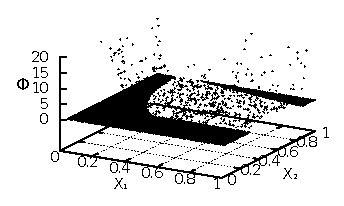
\includegraphics{fit_new.eps}}
%\end{minipage}
%\caption{$\Phi$ plot for 1000 randomly chosen individuals over the 2d design space of a two-objective constrained optimization problem (fig.\ref{case}) using the proposed penalization formulation (eq.\ref{penal2}).}
%\label{fit2}
%\end{figure}
 

\subsection{Metamodel assisted Evolutionary Algorithm}
\label{MAEApar}
Due to the involvement of costly evaluation tools (such as CFD tools to numerically predict flows in or around complex 3D geometries), solving engineering optimization problems using EAs may become very computationally demanding. The extensive, smart use of low-cost surrogate evaluation models (often referred to as "metamodels") during the optimization decreases substantially the number of calls to the computationally expensive, problem-specific evaluation code (CFD) making EAs a viable tool that can routinely be used to solve large-scale industrial optimization problems, with affordable wall clock time. Literature surveys on the use of metamodels within EAs can be found in papers \cite{LTT_2_020,Jin2002,LTT_2_027} or books \cite{KEANEbook}.


Polynomial regression, artificial neural networks, Gaussian processes etc. have all been used as metamodels.  Schemes based on different interactions between the metamodel and the problem-specific evaluation tool have been published. Hereafter, all of them will be referred to as MAEAs. Metamodels can be integrated in EAs in two ways the off- and the on-line trained metamodels. This types differ with respect of the timing of the metamodels training, i.e. whether this takes place before (off–line) or during (on–line) the evolution. In this thesis the on-line trained metamodels are in use \cite{LTT_2_018,LTT_2_029}. 
 
In on-line trained metamodels, for all but the first few generations, the metamodels are used to pre-evaluate the current population. Based on the outcome of approximate pre-evaluations (herein called inexact-pre-evaluation IPE), the few most promising individuals are identified and these solely undergo evaluation with the problem-specific evaluation tool to compute their "exact" objective function value(s), before proceeding to the next generation. The $(\mu,\lambda)$ MAEA used herein is sketched in fig.~\ref{MAEA}.


\begin{figure}[h!]
\centering
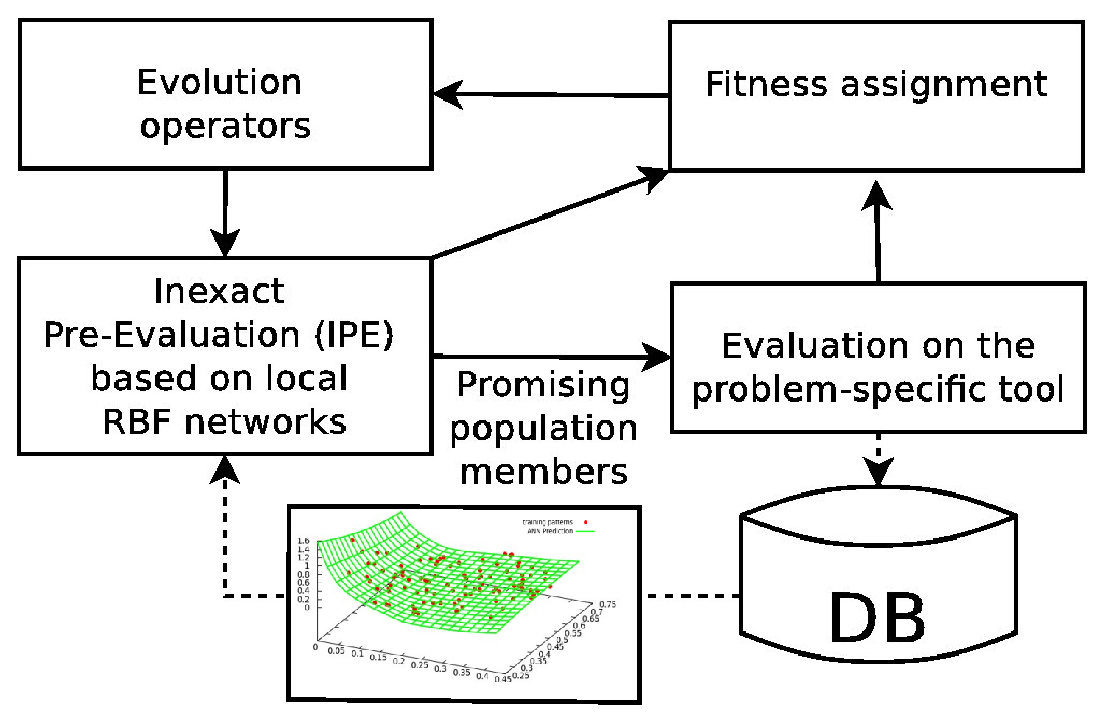
\includegraphics[width=90mm]{MAEA.eps} 
\caption{MAEA using on-line trained metamodels. The loop corresponds to a single EA generation. The so-called inexact pre-evaluation (IPE) phase, within the EA--based search, is used, as described in \cite{LTT_2_020,LTT_2_029}. }
\label{MAEA}
\end{figure}


\paragraph{Radial Basis Function networks RBFn}
In this thesis Radial Basis Function networks (RBFn) are used as metamodels although the method presented in the next chapters could be combined with any other type of metamodels. In more detail RBFn are artificial neural networks (ANN) with three neuron layers, (input,hidden and output) as shown in fig.\ref{rbf1} \cite{Haykin}. Signals propagate through the network in the forward direction, from the input to the output layer, by performing a nonlinear mapping (eq.\ref{RBFa}) followed by a linear one. The latter is related to the weight coefficients $w_l$ that must be computed during the training on a number of available patterns. An RBF network to be used within a MAEA should have $N$ input units, i.e. as many as the  design variables. The hidden layer includes $L$ nodes, associated with the so–called RBF centers $c^l$. At each hidden neuron a nonlinear mapping of the input signals to a single value is carried out using the radial-basis activation function $G:\Re^N \rightarrow \Re$, acting on the distance of input $x$ (eq.\ref{RBFa}) from the corresponding center $c^l \in \Re^N$.  In the current thesis the Gaussian activation is in use. 

\begin{eqnarray}
	G(u,r)=exp(\frac{-u^2}{r^2})
	\label{RBFa}
\end{eqnarray}  
where $u=\Vert x-c^l \Vert_2$ the distance from the corresponding $l^{th}$ RBF center.

\begin{figure}[h!]
\centering
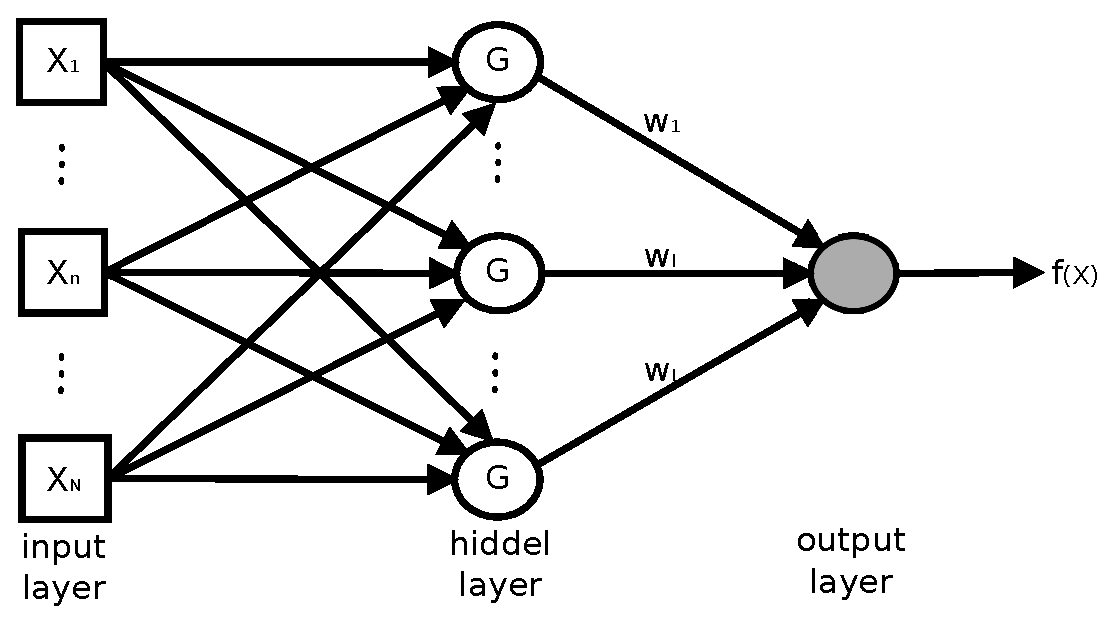
\includegraphics[width=90mm]{RBF.eps} 
\caption{Radial basis function network.}
\label{rbf1}
\end{figure}
The values that the radii or widths r take on may considerably affect the prediction abilities of the network; these are computed using heuristics,\cite{Haykin}. The output layer includes as many nodes as the responses of the network. The single response we are dealing with is expressed by the sum of the weighted output signals from the hidden neurons, as follows             
\begin{eqnarray}
	f(x)=\sum _1^K w_i*G(u(x_i),r)
\label{response}
\end{eqnarray}  

In the trivial case that number of hidden nodes ($K$) is equal to the number of training patterns ($T$), the choice of the $RBF$ centers is straightforward, i.e.
$\vec{c}^{(t)}\!\equiv\!\vec{x}^{(t)}$, $t\!\in\![1,T]$, ensuring
that the $T$ samples are exactly interpolated. 
In this case, the network training is reduced to the solution of a $T\!\times\!T$ symmetric linear system of equations, as follows,
%
\begin{equation}
    \sum_{t=1}^{T} w_t G(\|\vec{x}^{(t)}-\vec{c}^{(t)}\|_2)=
    \zeta^{(t)}
    \nonumber
\end{equation}

A common way to increase the network's generalization \cite{Pog1990, Tik76, Tik95} is by using less, appropriately selected, hidden nodes than the training patterns, i.e. selecting $K\!<\!T$. 
In this case, the selection of the $RBF$ centers is not trivial, as in the aforementioned case, and is of big importance since 
it strongly affects the prediction ability of the network. 
In \cite{LTT_2_029}, a selection scheme for the $RBF$ centers based on 
self-organizing maps ($SOMs$, \cite{Fri94a, Hayk1999}) was proposed. 
This practically comprises a two level learning scheme, namely the unsupervised and the supervised ones.
During the unsupervised learning, $SOMs$ (through their standard processes: 
competition, cooperation and adaptation) classify the training 
patterns into $K$ clusters.  
Each cluster gives a single $RBF$ center $\vec{c}^{(k)}$, considered to be representative of the cluster as a hole. The corresponding radius $r_k$ is computed using heuristics based on distances between the centers, \cite{Karay1997, LTT_2_029, Hayk1999, BenArc02}.
During the supervised learning, the synaptic weights are computed by minimizing the approximation error of the $RBF$ network over the training set, while considering smoothness requirements.
%
%\begin{figure}
%    \centering
%    \includegraphics[scale=0.6]{rbf-som.eps}
%    \caption{The two phases of an \RBF\ network training based on \SOMs:
%            (a) self-organized positioning of the \RBF\ centers (unsupervised 
%            learning) and (b) computation of the synaptic weights (supervised
%            learning.}
%    \label{f:rbfn-som}
%\end{figure}


The so--called \textit{Importance Factors} ($IFs$) \cite{LTT_2_018} can improve the prediction ability of the $RBFn$. Incorporating $N$ extra coefficients ($I_n, n\!=\!1,N$), the importance of each design parameter on the network response is quantified and exploited in order to increase the overall $RBFn$ prediction quality. High $I_n$ values indicate high sensitivity of the objective function in the vicinity of the design point under consideration with respect to the $n$-th input variable. The $IFs$ are computed by the $RBF$ network as a by-product of the training process and are used to improve the quality of the networks' output. 
In detail, each time an improved solution is computed by the $EA$ (index $b$, which stands for the current best), the corresponding local $RBF$ network is built and $N$ partial derivatives $\partial o^{(b)} / \partial x_{n}$ are computed using the network's closed-form expressions; by doing so, $\partial o^{(b)} / \partial x_{n}$ are the exact derivatives of an approximate function. 
Based on these derivatives, a weighted norm is introduced and used instead of the standard one (i.e. instead of eq. \ref{response}), as follows
%
\begin{equation}\label{e:IFcomp}
    \left\|\vec x^{(t)}-\vec c^{(k)}\right\|_{wei} =
    \sqrt{  \sum_{n=1}^N I_n\left(x_n^{(t)}-c_n^{(k)}\right)^2  }
	\mbox{,~where~~~~}
    I_n = { {\left|  {\partial o^{(b)}} \over {\partial x_n} \right|} 
          \over 
  { \sum_{i=1}^{N} \left| {\partial o^{(b)}} \over {\partial x_i} \right| } }
\end{equation}


\subsubsection{Inexact Pre--Evaluation algorithm}


The algorithm starts as a conventional $(\mu, \lambda)EA$ (by, exclusively, making use of the exact evaluation model) for the few starting generations until a user--defined minimum number of exact evaluations enter the $DB$. 
Then, the $IPE$ phase starts and, in subsequent generations, instead of evaluating the offspring population on the costly, problem--specific model, the following actions are taken:
\newcommand{\apprx}[1]{\tilde{#1}}
\begin{itemize}
\item[]{\bf Inexact evaluation:}
For each offspring, $\vec{x}\!\in\!P_{\lambda,g}$, the objective function values $\apprx{\vec{F}}(\vec{x})$, are approximated using a local metamodel trained on a small number of data selected from the $DB$. 
%
\item[]{\bf Screening:}
%>>>>
Based on the $\apprx{\vec{F}}(\vec{x})$ values, a provisional
$\phi$ value (denoted by $\apprx{\phi}$) is assigned to each
offspring.
%>>>>
\item[]{\bf Exact evaluation:}
%>>>>
For all $\vec{x}\!\in\!P_{e}$, the exact objective function values $\vec{F}(\vec{x})$ are computed and stored in the $DB$. 
Practically, this step, determines the $CPU$ cost of each generation.
%...................
\end{itemize}


\subsection{Hierarchical Evolutionary Algorithm}
Typically in engineering design a number of tools with different fidelity and cost (computational and/or economical) are available and used in different steps of the design procedure (fig.\ref{HMAEA} right). Relatively fast low fatality tools are used in the initial stages of the design in order to efficiently scan the design space and high fatality slow (and/or expensive with respect to licensed software or laboratory time) tools are used for the latter steps of design for fine-tuning. In case of turbo-machinery design, for example, a potential code can be used as a low fidelity tool followed by dense or coarse grid Euler codes, Navier-Stokes codes for a single flow passage or the full machine and finally actual laboratory test and adaptation cycles.    


\begin{figure}[h!]
\begin{minipage}[b]{1.0\linewidth}
 \centering
 \resizebox*{13cm}{!}{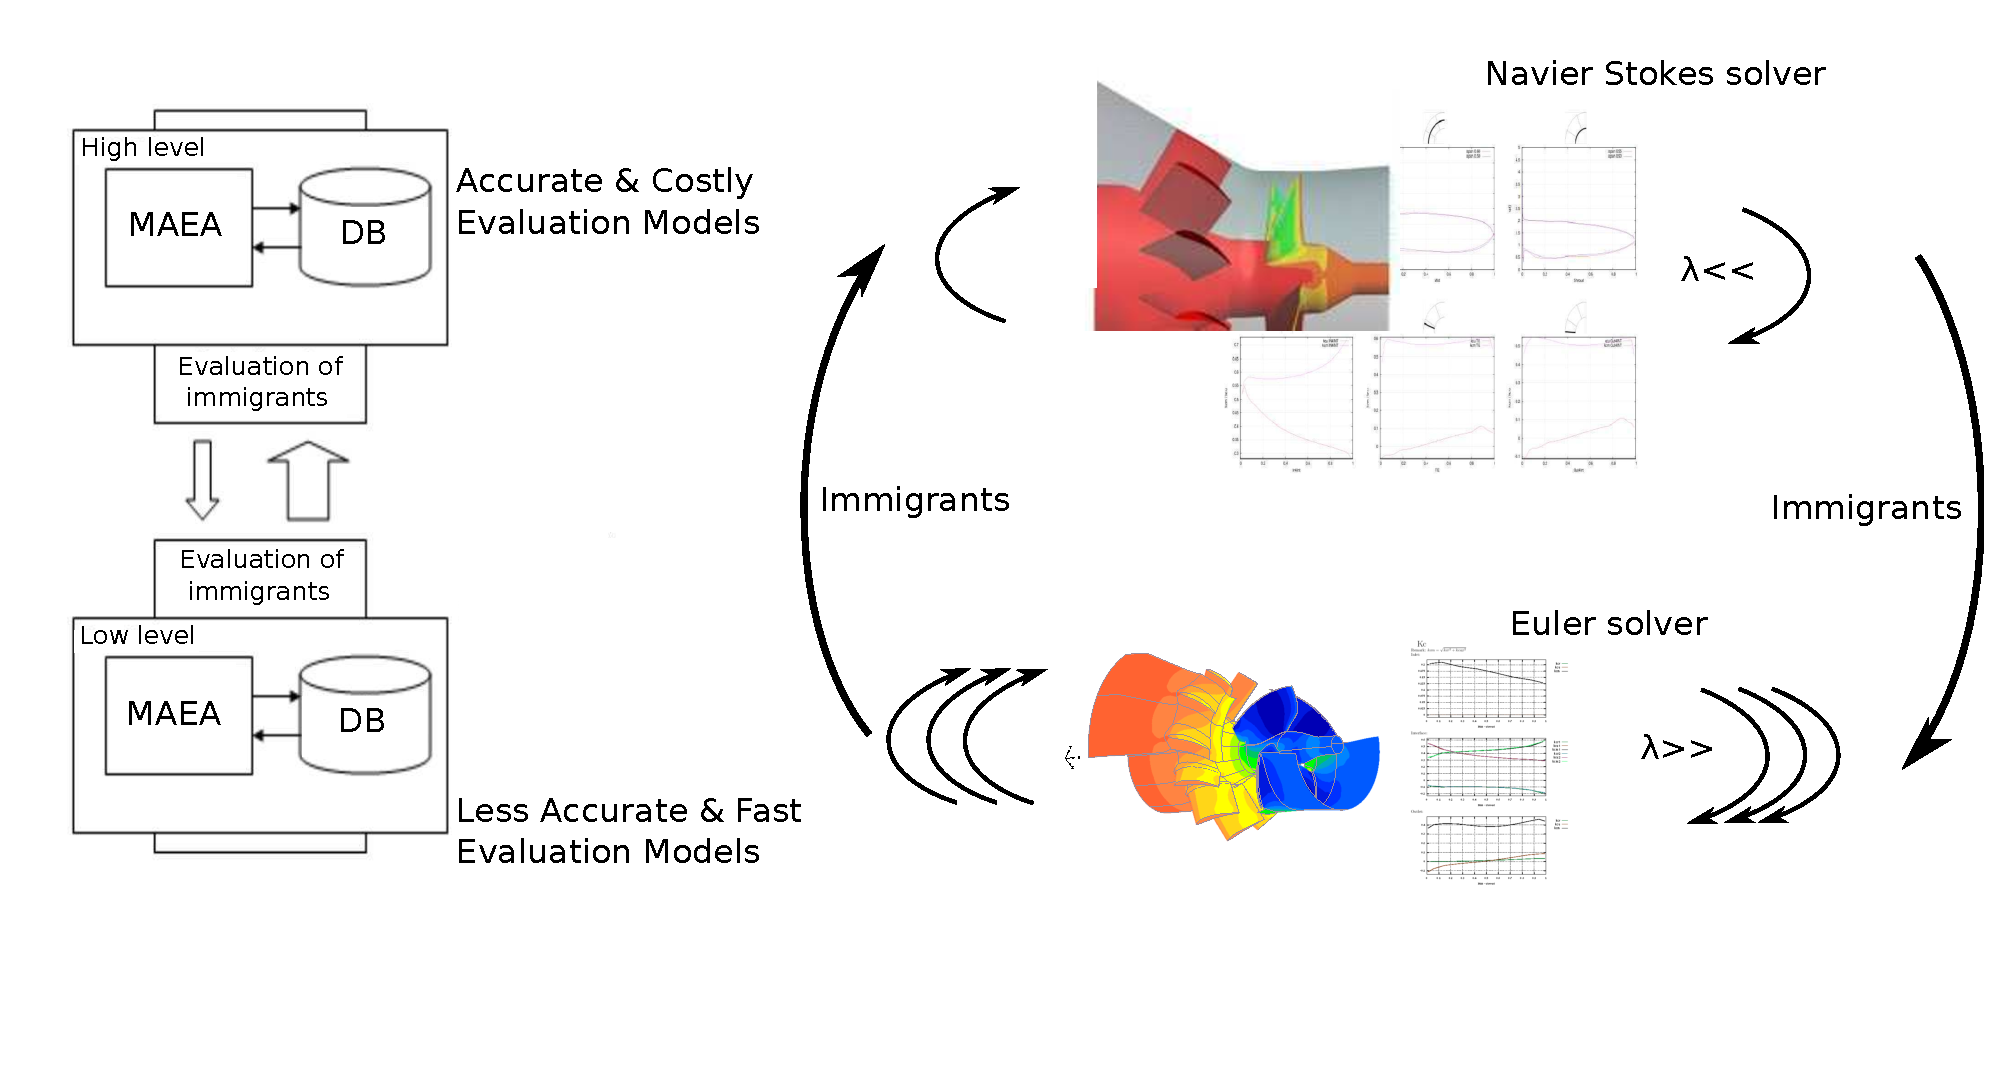
\includegraphics{handmade.eps}}
\end{minipage}
\caption{Left, schematic representation of a two level HMAEA (Hierarchical metamodel assisted evolutionary algorithm). High level is associated with the expensive and accurate tool and lower level with the cheap but not so accurate tool. Communication between the two level is possible in both directions including re-evaluation with the receiving levels evaluation tool. Right, example of two level design procedure as used in industry. A relatively big number of designs is evaluated with the Euler solver once a good design is located it is evaluated with the Navier-Stokes solver. Possible faults are identified, targets for the lower level are updated, that would result in the  elimination of the aforementioned faults, bye experienced designers.}
\label{HMAEA}
\end{figure} 
 
In order to exploit the availability of this tools Hierarchical evolutionary algorithms (HEA) where devised \cite{Herr1999, Sefr2000, Desid2003, LTT_2_031, LTT_3_092, LTT_2_036,
LTT_2_044, LTT_2_048, LTT_4_05}. HEA are enhanced EA variants which utilise a number of evolution Levels, each level assigned a different evaluation tool (fig.\ref{HMAEA} left). This multilevel search mechanism splits the computational burden among the levels. On the lower levels, a low cost exploration of the search space is carried out through global search methods, less demanding or less accurate evaluation tools or by even using reduced design variable sets, etc. On the other hand the higher levels undertake the fine-tuning part of the design procedure through denser parameterization, more accurate evaluation tools and/or stochastic or deterministic search methods. These levels mainly serve to refine immigrants from the lower levels. Intercommunication and two-way migrations of individuals between adjacent levels are necessary. The number of levels, the frequency of migration and the number of immigrants are user-defined parameters.

Respecting the aforementioned mechanisms HEAs can be categorized in three main types, that of course can be combined in any resulting schemes, namely the hierarchical evaluation,  search and parametrization (fig. \ref{allheas}). In hierarchical evaluation schemes the availability of evaluation tools with different cost and fidelity is exploited. In hierarchical search the combination of different search algorithms, thus combining their merits in a single optimization procedure, is achieved. And in hierarchical parametrization both course and detailed shape representations can be combined in order to both search the design space in an efficient/fast way via the course parametrization and locate the true optimum that might need the more detailed shape representation. 

\begin{figure}[h!]
    \centering
    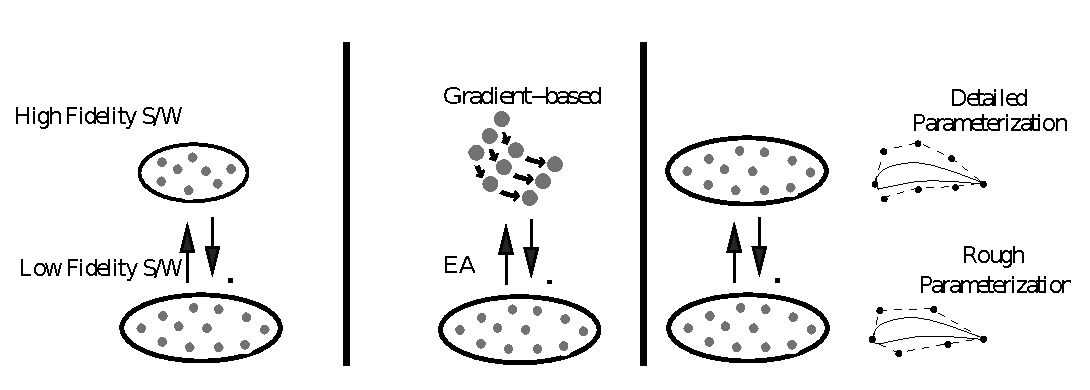
\includegraphics[scale=0.8]{multimodes.eps}
% ------------------------------------------------
    $\mbox{Hierarchical Evaluation~~~~~Hierarchical Search~~~~~~Hierarchical Parameterization}$
%   $\mbox{Hierarchical}~~~~~~~~~~~~~~~~
%    \mbox{Hierarchical}~~~~~~~~~~~~~~~~~~~~
%    \mbox{Hierarchical}$
%   \\
%   $~~~\mbox{ Evaluation }~~~~~~~~~~~~~~~~~~
%    \mbox{   Search   }~~~~~~~~~~~~~~~~~~~
%    \mbox{Parameterization}$
% ------------------------------------------------
    \caption{$HEAs$. Schematic representation of the three
            hierarchical schemes. Left: is the schematic representation of the hierarchical evaluation scheme where on the top level a costly but accurate evaluation model is used combined with small population sizes. On the lower level a fast but less accurate tool is used combined with larger populations in order to better search the design space. Middle: is the hierarchical search scheme where on the top level a gradient based method is used as search algorithm applied in a small number of individuals concurrently, in the case of MOO the weights, per objective, needed from the gradient based method are automatically commutated  based on the individuals position in the elite set. On the lower level an EA can be utilised in order to efficiently search the design space avoiding local optima. In the general form the evaluation software connected to the gradient based method is more computationally expensive since also the derivatives have to be computed, in case of an adjoint method \cite{LTTVKI04b} this costs approximately two calls of the lower level evaluation software. Left: is the hierarchical parametrization scheme where on the top level a detailed parametrization is utilized whereas on the lower level a rough parametrization is used. All this types can be combined or used separately at will utilizing two or more levels.}
    \label{allheas}
\end{figure}      
% ---------------------------------------------------------------------------
% ----------------------- end of thesis sub-document ------------------------
% ---------------------------------------------------------------------------